\index{Rosswog, Stephan}
\subsubsection{Compact Stellar Objects}
\label{GeoAstro:Rosswog}

\paragraph{Research Team}
Stephan Rosswog (Professor), Marius Dan (PhD student),
Traian Popescu (PhD student)\\


%%% give a very short (150 words description of your research area)

My research focuses on the physics and astrophysics of compact
stellar objects such as white dwarfs, neutron stars and black holes.
The related questions range from the formation of elements in the cosmos
over gravitational waves to stellar explosions such as supernovae or
gamma-ray bursts.

Gamma-ray bursts are the most violent explosions in the Universe
since the Big Bang. They come in two flavours: as {\em long}
bursts that are accompanied with the explosion of very massive
stars and as {\em short} bursts. After nearly four decades of
in intense research, in summer 2005 for the first time an
``afterglow'' of the so far elusive short gamma-ray bursts
could be detected. Most of the observed properties of both the explosion
itself and its host galaxy suggest that it is produced
when two compact objects, either a double neutron star
system or a binary system containing a neutron star and a black
hole, collide with each other. The observed X-ray activity long after the
burst, however, represents a stumbling block for current theoretical models.

\paragraph{Highlights}

%%% give a short (500 words)description of the research highlights.
%1 figure costs 100 words

%NSM
Several {\em double neutron star systems} are known in our Galaxy.
They serve as
probes for fundamental physics in several ways. The neutron star
masses that can be inferred very accurately from general relativistic effects
in the binary orbital motion are the tightest available constraints on
the strong interaction. Moreover, the orbital decay due to the emission
of gravitational waves has been measured and provides the best available
test to the so-called ``quadrupole-approximation'' of Einsteins theory of
General
Relativity. The decay of the binary orbit leads to a final coalescence
of the two neutron stars and to the release a tremendous amount
($\sim 3\cdot 10^{53}$ erg) of gravitational binding energy.\\
Neutron stars are known to possess strong magnetic fields, but a global
simulation of a magnetic neutron star collision is a prime computational
challenge. In a concerted effort, we (Daniel Price, University of Exeter,
UK and S.R.) have recently developed a new numerical method
(Smoothed Particle Hydrodynamics  with Euler-potentials) that fulfills
the ``$\vec\nabla \cdot \vec{B}= 0$''-constraint on the magnetic field by
construction. With this method we were able to perform the world-wide first
global magnetohydrodynamics simulations of a neutron star collision. The main
result is that existing magnetic fields are tremendously amplified
within the first milli-seconds of the collision. These extremely large
magnetic fields are a prime candidate to launch the ultra-relativistic outflow
(bulk Lorentz factors of several hundred) that is needed to explain the
observed properties of gamma-ray bursts. The first results of our
simulations were published as the cover story of {\em Science}
\cite{Rosswog1}. Further publications on this topic are currently in
preparation.\\
In a separate work I have proposed an analytical model to explain the
observed long-term X-ray activity \cite{Rosswog2}.

\begin{figure}[ht]
  \begin{center}
    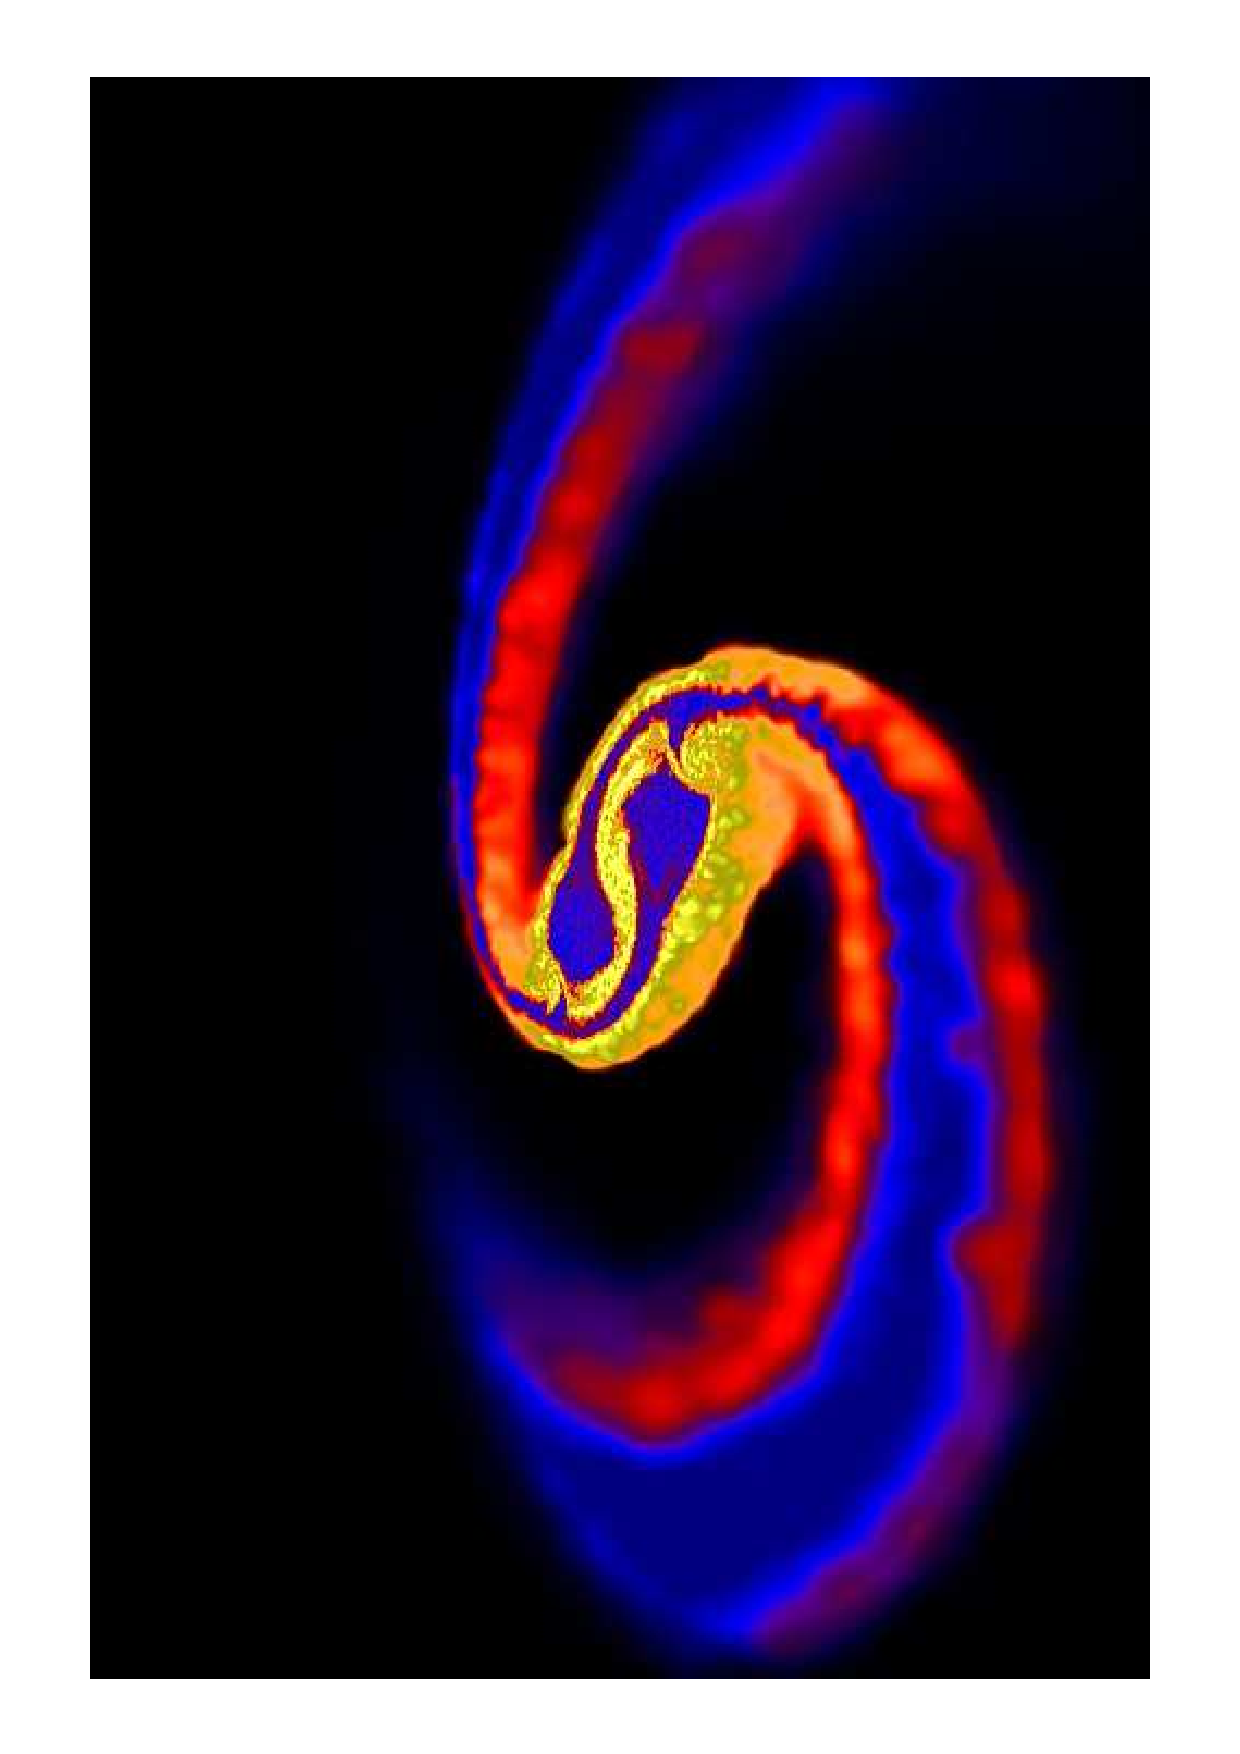
\includegraphics[height=\hsize, angle=270]{Rosswog/Rosswog_2006.pdf}
    \mycaption{Coalscence of two magnetised neutron stars. The snapshot
               shows the matter distribution 2 milliseconds after the merger,
               colour-coded is the strength of the magnetic field.}
    \label{NSM_mag}
  \end{center}
\end{figure}

\noindent Suggestive evidence has accumulated that the globular star
clusters that surround the Milky Way and other galaxies harbour
so-called ``{\em intermediate-mass black holes}'' of several hundred to
several thousand solar masses. We (Enrico-Ramirez-Ruiz, Institute for
Advanced Studies Princeton, USA and S.R.) have analyzed tidal disruption
processes of white dwarf stars near such intermediate-mass
black holes as a diagnostic for the existence of this hypothetical breed
of black holes. We find that for close encounters tidal interaction can
trigger a thermo-nuclear explosion of the white dwarf. Long-lived intense
accretion activity will be the main signature in the aftermath of such a
disruption. The results of our recent investigation of this topic
are currently prepared for publication.

\paragraph{Activities}
\begin{itemize}
\item Organisation of the summer meeting of the Rat Deutscher Sternwarten
  (RDS) at IUB (18.9.2006)
\item Coordination and formulation of a proposal for a DFG priority program
      ``Computational Astrophysics (CompAs)'' (together with M. Br\"uggen;
      coordinator of the proposal: S. Rosswog)
\end{itemize}

\paragraph{Collaborations}
\begin{enumerate}
\item {\sl Istituto Nazionale di Fisica Nucleare, Catania, Italy}\\
Dr. Marcello Baldo
\item {\sl University of Exeter, UK} \\
Dr. Daniel Price
\item {\sl Institute for Advanced Study, Princeton, USA} \\
Prof. Dr. Enrico  Ramirez-Ruiz
\item {\sl University of Leicester, UK} \\
Dr. Richard West
\end{enumerate}

\paragraph{Other Support Grants }
\begin{enumerate}
% list the grants you have received in 2005, if none have been received, plese delete this
\item 50 000 CPU hours on the JUMP supercomputer at the H\"ochstleistungsrechenzentrum J\"ulich
\end{enumerate}


% subsection.
\paragraph{Awards, Prizes}
\begin{enumerate}
\item ``Expert of International Standing'' of the Australian Research Council (ARC)
\end{enumerate}

%\paragraph{Publications}
\nocite{Rosswog1} \nocite{Rosswog2} \nocite{Rosswog3}
\nocite{Rosswog4} \nocite{rosswog5}
%
